\documentclass[tikz,border=8pt]{standalone}
\usepackage{amsmath,amssymb}
\usetikzlibrary{arrows.meta,calc}
\definecolor{TargetBlue}{HTML}{2364AA}
\definecolor{NuisanceOrange}{HTML}{E6862A}
\definecolor{EfficientGreen}{HTML}{278A64}
\definecolor{NeutralGray}{HTML}{68717C}
\begin{document}
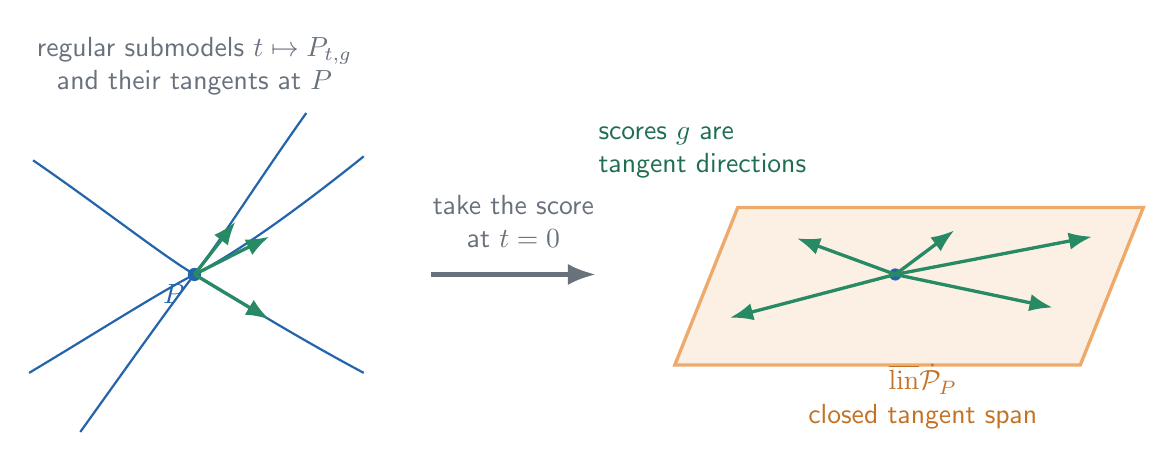
\begin{tikzpicture}[font=\sffamily, >=Latex]
  % Left panel: several regular paths through the same distribution.
  \begin{scope}[xshift=-4.7cm]
    \draw[TargetBlue, thick]
      (-2.1,-1.25) .. controls (-1.15,-0.68) and (-0.45,-0.23) .. (0,0)
      .. controls (0.55,0.28) and (1.3,0.82) .. (2.15,1.5);
    \draw[TargetBlue, thick]
      (-1.45,-2.0) .. controls (-0.82,-1.12) and (-0.28,-0.36) .. (0,0)
      .. controls (0.32,0.41) and (0.8,1.18) .. (1.42,2.05);
    \draw[TargetBlue, thick]
      (-2.05,1.45) .. controls (-1.15,0.83) and (-0.42,0.25) .. (0,0)
      .. controls (0.52,-0.31) and (1.25,-0.77) .. (2.15,-1.25);

    \coordinate (P) at (0,0);
    \fill[TargetBlue] (P) circle (2.4pt);
    \node[below left, text=TargetBlue] at (P) {$P$};
    \draw[->, very thick, EfficientGreen] (P) -- (0.95,0.48);
    \draw[->, very thick, EfficientGreen] (P) -- (0.52,0.67);
    \draw[->, very thick, EfficientGreen] (P) -- (0.95,-0.57);
    \node[text=NeutralGray, align=center] at (0,2.65)
      {regular submodels $t\mapsto P_{t,g}$\\and their tangents at $P$};
  \end{scope}

  % The score map turns path derivatives into elements of L2(P).
  \draw[->, NeutralGray, ultra thick] (-1.7,0) -- (0.4,0)
    node[midway, above=2mm, align=center] {take the score\\at $t=0$};

  % Right panel: scores and their closed linear span.
  \begin{scope}[xshift=4.2cm]
    \fill[NuisanceOrange!12] (-2.8,-1.15) -- (2.35,-1.15) -- (3.15,0.85) -- (-2.0,0.85) -- cycle;
    \draw[NuisanceOrange!70, very thick] (-2.8,-1.15) -- (2.35,-1.15) -- (3.15,0.85) -- (-2.0,0.85) -- cycle;
    \coordinate (Q) at (0,0);
    \fill[TargetBlue] (Q) circle (2.2pt);
    \foreach \x/\y in {-2.1/-0.55,-1.25/0.46,0.75/0.56,2.0/-0.42,2.5/0.48}{
      \draw[->, very thick, EfficientGreen] (Q) -- (\x,\y);
    }
    \node[text=EfficientGreen!80!black, align=left] at (-2.45,1.55)
      {scores $g$ are\\tangent directions};
    \node[text=NuisanceOrange!85!black, align=center] at (0.35,-1.55)
      {$\overline{\operatorname{lin}}\dot{\mathcal P}_P$\\closed tangent span};
  \end{scope}
\end{tikzpicture}
\end{document}
